\documentclass[14pt,onecolumn,a4paper]{article}
\usepackage[a4paper, mag=1000, left=2cm, right=2cm, top=2cm, bottom=2cm, headsep=1cm, footskip=1cm]{geometry}
\usepackage[T2A]{fontenc}
\usepackage[utf8]{inputenc}
\usepackage[english,russian]{babel}
\usepackage{indentfirst}
\usepackage[dvipsnames]{xcolor}
\usepackage{listings} 
\usepackage{caption}
\usepackage{amsthm}
\usepackage{amsmath}
\usepackage{amssymb}
\usepackage{array}
\usepackage{float}
\usepackage{afterpage}
\usepackage{graphicx}
\usepackage{placeins} % For \FloatBarrier
%\usepackage{newtxtext} % Times New Roman font
\usepackage[
citestyle=alphabetic-verb,
bibstyle=bibfiles/gost-numeric
]{biblatex}
\addbibresource{cite.bib} % Specify the bibliography file
\usepackage[colorlinks, linkcolor=black, urlcolor=black, citecolor=black]{hyperref}
\newcommand{\notes}[3][\empty]{%
    \noindent Оценка\vspace{5pt}
        {\rule{#3}{0.5pt}\\}
}
\newtheorem{definition}{Определение}[section] % This makes the definition counter reset at each new section
\DeclareCaptionFont{white}{\color{white}} 
\DeclareCaptionFormat{listing}{\colorbox{gray}{\parbox{\textwidth}{#1#2#3}}}
\captionsetup[lstlisting]{format=listing,labelfont=white,textfont=white}
\lstset{% Собственно настройки вида листинга
inputencoding=utf8, extendedchars=\true, keepspaces = true, % поддержка кириллицы и пробелов в комментариях
language=Pascal,            % выбор языка для подсветки (здесь это Pascal)
basicstyle=\small\sffamily, % размер и начертание шрифта для подсветки кода
numbers=left,               % где поставить нумерацию строк (слева\справа)
numberstyle=\tiny,          % размер шрифта для номеров строк
stepnumber=1,               % размер шага между двумя номерами строк
numbersep=5pt,              % как далеко отстоят номера строк от подсвечиваемого кода
backgroundcolor=\color{white}, % цвет фона подсветки - используем \usepackage{color}
showspaces=false,           % показывать или нет пробелы специальными отступами
showstringspaces=false,     % показывать или нет пробелы в строках
showtabs=false,             % показывать или нет табуляцию в строках
frame=single,               % рисовать рамку вокруг кода
tabsize=2,                  % размер табуляции по умолчанию равен 2 пробелам
captionpos=t,               % позиция заголовка вверху [t] или внизу [b] 
breaklines=true,            % автоматически переносить строки (да\нет)
breakatwhitespace=false,    % переносить строки только если есть пробел
escapeinside={\%*}{*)}      % если нужно добавить комментарии в коде
}
\usepackage{acronym}
\newcommand{\addabbreviation}[2]{%
    \entry{#1}{#2}
}

% Adjust section and subsection font size and style
\usepackage{titlesec}
\titleformat*{\section}{\fontsize{14pt}{17pt}\selectfont\bfseries}
\titleformat*{\subsection}{\fontsize{14pt}{17pt}\selectfont\bfseries}

\begin{document}
\fontsize{14pt}{17pt}\selectfont
% Переоформление некоторых стандартных названий
%\renewcommand{\chaptername}{Научно-исследовательская работа}
\def\contentsname{Содержание}

% Оформление титульного листа
\begin{titlepage}
\begin{center}
\textbf{Федеральное государственное автономное образовательное учреждение высшего образования\\
«РОССИЙСКИЙ УНИВЕРСИТЕТ ДРУЖБЫ НАРОДОВ»
(РУДН)
\\[5mm]
Факультет физико-математических и естественных наук\\[2mm]
Кафедра математического моделирования и искусственного интеллекта}
\end{center}

\vfill

\begin{flushleft}
Основное учебное подразделение: факультет физико-математических и естественных наук\\
Направление/специальность: 02.03.01 Математика и компьютерные науки
\end{flushleft}

\begin{center}
\textbf{ОТЧЁТ\\[3mm]
о прохождении учебной практики\\[3mm]
«Научно-исследовательская работа (получение первичных навыков научно-исследовательской работы)» 
\\[20mm]
}
\end{center}

\hfill
\begin{center}
Абу Сувейлим Мухаммед Мунифович\\
\end{center}

\begin{flushleft}
Курс, группа: 3, НКНбд-01-21\\[3mm]
Место прохождения практики: научные центры института прикладной математики и телекоммуникаций \\[6mm]
Сроки прохождения с «15» апреля 2024 г. по «15» июня 2024 г. 
\end{flushleft}

\vfill

\begin{minipage}{7cm}
{Руководители практики:\\[3mm]
от РУДН Фомин М.Б., к.ф.-м.н, доцент\\ 
от организации (предприятия)  Самуйлов К.Е., директор ИКНиТ}
\end{minipage}

\vspace{12mm}	
\notes{1}{0.5\textwidth}

\vfill

\begin{center}
 Москва, 2024 г.
\end{center}

\end{titlepage}


% Содержание
\tableofcontents
\newpage
\section{Введение}

\subsection{Цель работы}


Согласно программе учебной практики направления подготовки 02.03.01 «Математика и компьютерные науки», целями практики являются:
\begin{itemize}
   \item формирование профессиональных навыков в проведении научных исследований;
   \item формирование навыков использования современных научных методов для решения научных и практических задач;
   \item формирование практических навыков написания вспомогательных программных комплексов для проведения вычислительных экспериментов;
   \item формирование общекультурных, общепрофессиональных и профессиональных компетенций в соответствии с ОС ВО РУДН;
   \item формирование навыков оформления и представления результатов научного исследования;
   \item формирование навыков работы с источниками данных.
\end{itemize}

Для достижения целей в рамках учебной практики был выполнен обзор публикаций российских и международных научных изданий по теме выпускной квалификационной работы (ВКР) бакалавра, которая определена как «Анализ тональности финансовых новостей».

Время проведения учебной практики – 15.04.2024г.-15.06.2024г., место проведения практики – Отдел технической поддержки пользователей (департамент технологических и информационных ресурсов) РУДН и научные центры института компьютерных наук и телекоммуникаций РУДН.

Последовательность прохождения практики, перечень работ, выполненных в процессе практики (таб.~\ref{tabl:1}):
\begin{center}
\begin{table}[H]
\centering
\caption{Последовательность прохождения практики, перечень работ, выполненных в процессе практики}
\label{tabl:1}
\begin{tabular}{|c|m{5cm}|m{6cm}|c|}
\hline
№ п/п & Работы и мероприятия & Пояснение & Сроки выполнения \\
\hline
1 & Установочное занятие & Инструктаж по безопасности труда и правилам пожарной безопасности при выполнении лабораторных и практических работ. Обсуждение задания на практику. Разъяснение требований к заполнению & 15.04.2024 \\
\hline
2 & Подбор материалов & Подбор материалов для написания НИР. & 16.04.-18.04.2024 \\
\hline
3 & Оформление введения и теоретической части НИР. Накопление, систематизация и анализ теоретических и прикладных материалов. Составление библиографии по основным источникам. & Систематизация и обобщение научной и учебной литературы. & 19.04-22.04.2024 \\
\hline
4 & Подготовка материалов НИР. Практическая часть. & Изучение научной и учебной литературы. & 23.04.-03.05.2024 \\
\hline
5 & Подготовка материалов НИР. Практическая часть. & Проведение развернутого эксперимента для НИР. Обсуждение результатов эксперимента. & 04.05.-07.05.2024 \\
\hline
6 & Написание второго раздела НИР. & Сбор данных для дальнейшей реализации алгоритмов. & 08.05.-18.05.2024 \\
\hline
7 & Подготовка отчета и дневника по практике. & Разработка реализации алгоритмов, реализующих решение задачи НИР. & 20.05-08.06.2024 \\
\hline
8 & Подготовка отчета и дневника по практике. & Собеседование с научным руководителем и руководителем практики по содержанию отчета и дневника по практике. & 10.06-11.06.2024 \\
\hline
9 & Сдача отчета и дневника по практике руководителю практики. & Прикрепит нужные документы и файлы к ТУИС. & 15.06.2024 \\
\hline
\end{tabular}
\end{table}
\end{center}


\subsection{Задание}

Заданием является анализ тональности текста и состоит оно из двух частей. Получив текст на английском языке, модель должна определить оценку тональности текста и к какому объекту в тексте тональность относится. Рассмотрим следующий пример: \flqq Apple stocks went up by 10\% on Monday, as reported by TASS\frqq. В тексте две сущности: \flqq Apple\frqq \vspace{1pt} и \flqq TASS\frqq, поэтому программа должна вывести два двухэлементных кортежа: (Apple, Positive) и (TASS, Negative). На самом деле, в рамках НИР было достаточно определить оценку тональности, но было принято решение определить объекты/сущности в тексте.  

\section{Основная часть} 
\subsection{Теоретическая часть}


Анализ тональности текста – это подраздел обработки естественного языка (NLP), целью которого является классификация текста по тональности. Тональность — это мнение, отношение и эмоции автора по отношению к объекту, о котором говорится в тексте \cite{Samigulin2021}. Также объекты можно разделить на разные категории. В Python библиотеке SpaCy, одна из самых распространнейных библиотек в сфере NLP, существует 18 категорий объектов, такие как человек (PERSON); национальности, религиозные или политические группы (NORP); здания, аэропорты, автомагистрали, мосты (FAC), компании, агентства, учреждения (ORG) и так далее \cite{spaCy}. 
Прежде чем начать, нужно дать определение нескольким важным терминам.

\begin{definition}
    Мнение - это четырехэлементный кортеж
    \begin{align*}
        (g, s, h, t),
    \end{align*}
    где $g$ - целевой объект тональности (sentiment target), $s$ - тональность мнения относительно объекта $g$ (sentiment), $h$ - носитель мнения (лицо или организация, придерживающиеся мнения; opinion holder), а $t$ - время, когда мнение было выражено (time). (13, \cite{10.5555/3110802})
\end{definition}

Отсутствие хотя бы одного элемента из кортежа резко ухудшает качество информации. Например, мнение, имеевшее место 5 лет назад, в большинстве случаев является  неактуальным по сравнению с мнением на сегодня. И если не указать этот временной отрезок, то информация может оказать недостоверной. Также имеет большое значение, кто является носителем такого мнения, например, презедент РФ или средестатистический гражданин РФ.

Стоит отметить, что у мнения есть объекты/сущности. В предложении с несколькими объектами нужно определить конкретный объект для каждого положительного или отрицательного мнения. Рассмотрим в качестве примера следующее предложение: \flqq Apple stocks went up on Monday,  while Microsoft stocks went down\frqq. Оно имеет как позитивную,так и негативную тональность. Объект с позитивной тональностью - Apple, объект с негативной тональностью - Microsoft.

\begin{definition}
Целевой объект тональности, также известный как целевой объект для выражения мнения - это объект, сущность, часть или атрибут объекта, в отношении которого было выражено мнение с эмоциональной окраской.(14, \cite{10.5555/3110802})
\end{definition}

Существуют различные формулировки определений понятий \flqq мнение/тональность\frqq, отличающиеся составом, например,
Лю определил мнение как кортеж из 5 элементов: <носитель тональности, объект тональности, аспект/атрибут объекта тональности, оценка тональности, время, когда мнение было выражено>\cite{inbook}.

В этой научно-исследовательской работе нас интересует оценка тональности (позитивная, негативная, нейтральная) и объект тональности финансовых новостей.

Анализ тональности финансовых новостей - это двухэтапная задача. Первая - это задача извлечения именованных сущностей (NER) из текста и классификация их по категориям, таким как имена людей, названия организаций, даты, местоположения, суммы денег и другие типы специфических объектов \cite{microsoft}. Вторая - это  задача  анализа и классификации тональности в тексте по трем категориям: Positive (Положительный), Negative (Отрицательный), Neutral (Нейтральный). Такая задача называется Target (Aspect) Based Sentiment Analysis (TBSA или ABSA). В переводе на русский язык это звучит как анализ тональности/эмоциональности на основе аспектов. ABSA как тема исследования получила особое внимание на соревновании/воркшопе SemEval-2014 \cite{pontiki-etal-2014-semeval}, где она была впервые представлена в качестве четвертого задания этого соревнования и снова появилась на SemEval-2015 \cite{pontiki-etal-2015-semeval} и SemEval-2016 \cite{pontiki-etal-2016-semeval} в последующие годы. 

С появлением технологии трансформеров в 2017 г. \cite{GoogleBrain} в области обученных языковых моделей был сделан большой шаг вперед, пример таких технологий - generative pre-trained transformer (GPT) (\cite{radford2018improving}) и BERT \cite{devlin-etal-2019-bert}. В этой научно-исследовательской работе мы будем использовать механизм модели Local Context Focus (LFC, механизм фокусировки на локальном контексте) \cite{Zeng2019LCFAL}, использующий блоки внимания (Multi-head Self-Attention) и BERT. Для имплементации этой модели мы выбрали Python фреймворк pyABSA \cite{YangL22}, который содержит множество моделей ABSA и упрощает процесс программирования моделей и визуализации графиков обучения и тестирования моделей. 

При осуществлении анализа  термины \flqq настроение\frqq, \flqq тональность\frqq \vspace{1pt} и \flqq сентиментальность\frqq \vspace{1pt} будут использованы взаимозаменяемо. Для обозначения первой задачи вместо NERO используется термин Aspect Term Extraction (извлечение аспектного термина, APE), для задачи классификации используется термин Aspect Polarity Classification (классификация полярности аспектов, APC). Также не проводится разграничение между ABSA и TBSA.

\subsubsection{Извлечение именованных сущностей Named Entity Recognition}

В модели Fast LFC прямо не применяются какие-либо методы для извлечения именованных сущностей. Для этого в Fast LFC ипользуются слои Context features Dynamic (CDM) и/или Mask Context Features Dynamic Weighted (CDW). Слой CDM фокусируется на локальном контексте, маскируя выходные представления менее семантически относящихся к контексту слов. Слой CDW ослабляет характеристики менее семантически относительных контекстных слов.


% Figure 1
\begin{figure}[htbp]
    \centering
    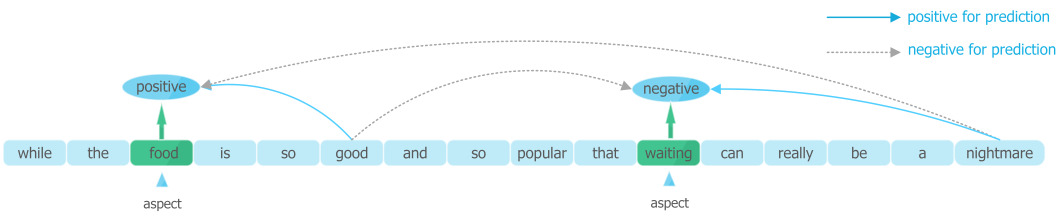
\includegraphics[width=1\linewidth]{images/Different influence of context words on sentiment polarity prediction.png}
    \caption{Влияние контекста на предсказание тональности. Показано только влияние типичных сентиментальных контекстных слов. \cite{Zeng2019LCFAL}}
    \label{fig:context-words-1}
\end{figure}

\vspace{3mm}

% Figure 2
\begin{figure}[htbp]
    \centering
    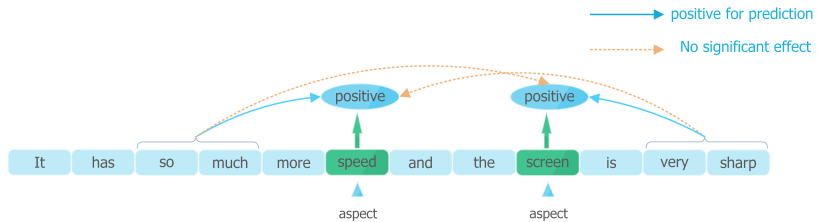
\includegraphics[width=1\linewidth]{images/Different influence of context words on sentiment polarity prediction2.png}
    \caption{Влияние контекста на предсказание тональности. Показано только влияние типичных сентиментальных контекстных слов. \cite{Zeng2019LCFAL}}
    \label{fig:context-words-2}
\end{figure}

\FloatBarrier % Ensures figures are placed before this point
Если рассматривается только задача извлечения именованных сущностей, то для этого существуют более простые варианты/методы в библиотеках spaCy и NLTK.   

\subsubsection{Анализ тональности текста по отношению к объекту}

В Fast LCF модели используется версия DeBERTA от BERT. BERT (и его разные версии DeBERTA, RoBERTa) позволяет получать высокие (state-of-the-art) результаты по задачам NLP, такие как оценка GLUE, составляющая 80.5\% (абсолютное улучшение на 7.7\%); точность MultiNLI до 86,7\% (абсолютное улучшение на 4,6\%), оценка F1 ответов на вопросы SQuAD v1.1 до 93,2\% (абсолютное улучшение на 1,5\%) и SQuAD v2.0 Тестируют F1 до 83,1\% (абсолютное улучшение на 5,1\%) \cite{Devlin2019BERTPO}.

В отличие от Open AI GPT и ELMo, BERT одновременно рассматривает как левую, так и правую сторону контекста. Хотя ELMo тоже использует двухнаправленный подход, но это лишь конкатенация контекстуальных представлений каждого токена слева направо и справа налево. С другой стороны, BERT устраняет ограничение однонаправленности, используя предварительную цель обучения “замаскированной языковой модели” (masked language model, MLM), вдохновленную задачей Клозе 1953 г. \cite{Devlin2019BERTPO}. 

% Figure 3
\begin{figure}[!ht]
    \centering
    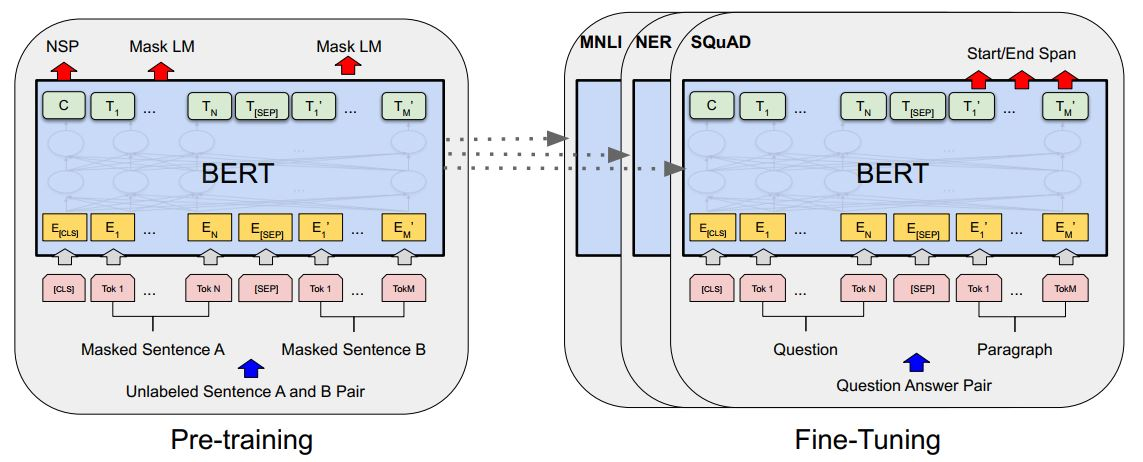
\includegraphics[width=1\linewidth]{images/Overall pre-training and fine-tuning procedures for BERT.JPG}
    \caption{Общие процедуры pre-training и fine-tuning для BERT. Помимо слоя вывода, для pre-training и fine-tuning используются одни и те же архитектуры. Одни и те же параметры предварительно обученной модели используются для инициализации моделей для различных (down-stream) задач, выполняемых в нисходящем потоке. Во время fine-tuning все параметры настраиваются точно. [CLS] - это специальный символ, добавляемый перед каждым примером ввода, а [SEP] - специальный разделительный токен (например, для разделения вопросов и ответов).}
    \label{fig:bert-architecture-1}
\end{figure}

BERT использует вложения/эмбеддинги WordPiece со словарным запасом в 30 000 токенов. Первый токен каждой последовательности (текста) всегда является специальным классификационным токеном (special classification token, [CLS]). Конечное скрытое состояние/пространство (hidden state), соответствующее этому токену, используется в качестве представления совокупной последовательности для задач классификации. Другими словами, токен [CLS]  - это вся последовательность ввода или предложение в виде вектора. Пары предложений объединяются в единую последовательность. BERT различает предложения двумя способами. Во-первых, BERT разделяет предложения специальным символом ([SEP]). Во-вторых, BERT добавляет к каждому символу выученный эмбеддинг (learned embedding), указывающий, принадлежит ли он предложению A или предложению B. Как показано на рисунке 1, E обозначает вложение входных данных (input embedding) , \[C \in 	\mathbb{R}^H\] - специальный токен [CLS] конечного скрытого вектора, а \[T_i \in 	\mathbb{R}^H\] - конечный скрытый вектор для i-го входного токена.

\subsection{Листинг программы}

Перед имплементацией модели обратим внимание на структуру набора данных. В отличии от обычной задачи классификации эмоциональной окраски текста, где у нас есть string текст и бинарный класс либо многоклассовый класс меток (позитивных, негативных и/или нейтральных), в задаче анализа тональности текста на основе аспектов ABSA также есть класс объектов тональности. Иногда добавляется класс категорий объектов и класс атрибутов/аспектов для каждого объекта. Это значительно усложняет задачу классификации, так как 
это приводит к отсутствию стандартной структуры набора данных. В этой НИР мы придерживаемся структуры набора данных, использованных в воркшопах на SemEval 2014, SemEval 2015 и SemEval 2016. 

\begin{lstlisting}[label=listing1, caption=Структура набора данны]
Forward O -999
Markets O -999
Commision O -999
allows O -999
national B-ASP Neutral
commodity I-ASP Neutral
bourses I-ASP Neutral
to O -999
impose O -999
different O -999
deal O -999
charges O -999
\end{lstlisting}

В наборе следующие ATE метки:
\begin{itemize}
    \item 'O' (Outside) - указывает, что слово не является частью аспектного термина.
    \item 'B-ASP' (Beginning of Aspect Term) - указывает на начальное слово аспектного термина.
    \item 'I-ASP' (Inside Aspect Term) - указывает, что слово находится внутри аспектного термина, т.е. является частью аспектного термина.
\end{itemize}
Метки тональности после каждого аспекта:
\begin{itemize}
    \item 'Positive' - положительное значение/слово.
    \item 'Negative' - отрицательное.
    \item 'Neutral' - нейтральное.
    \item '-900' - фиктивное значение (placeholder/dummy value).
\end{itemize}

Переходим к имплементации модели анализа тональности финансовых новостей на основе аспектов используя Python фреймворк pyABSA. Выполнение кода шаг за шагом позволяет получить те же самые результаты, полученные в этой работе. Модель была обучена на Kaggle Notebook с использованием видеокарты NVIDIA Tesla T4.

Во-первых, нужно установить фреймворк pyABSA и пакет autocuda для обучения модели на видеокартах от NVIDIA. 
\begin{lstlisting}[label=listing1, caption=установка фреймворка, language = Python]
!pip install pyabsa -U
!pip install autocuda
\end{lstlisting}

Во-вторых, мы импортируем необходимые библиотеки.
\begin{lstlisting}[label=listing2, caption=установка фреймворка, language = Python]
import autocuda
import random
from pyabsa import AspectTermExtraction as ATEPC
# Put your dataset into integrated_datasets folder, it this folder does not exist, you need to call:
from pyabsa import download_all_available_datasets
from pyabsa import DatasetItem
from pyabsa import ModelSaveOption, DeviceTypeOption
# MetricVisualizer to create graphs
from metric_visualizer import MetricVisualizer
import warnings
import torch
#to insure the models works use these versions
from pyabsa import __version__
assert __version__ >= '1.8.20'

from metric_visualizer import __version__
assert __version__ >= '0.4.0'
\end{lstlisting}

Далее, скачаем любой из наборов данных доступных в фреймворке либо прикрепляем собственный набор данных к директории. Так как нас интересуют финансовые новости, выбираем набор данных finNews.
\begin{lstlisting}[label=listing3, caption=Выбар набора данных, language = Python]
warnings.filterwarnings('ignore')
download_all_available_datasets()
dataset = DatasetItem(r"integrated_datasets/atepc_datasets/133.finNews")
\end{lstlisting}

Существует разные модели на разных архитектурах. Больше всего для нас подходит модель Fast LCF.
\begin{lstlisting}[label=listing4, caption=Выбар модели, language = Python]
config = (
    ATEPC.ATEPCConfigManager.get_atepc_config_english()
)  # this config contains 'pretrained_bert', it is based on pretrained models
config.model = ATEPC.ATEPCModelList.FAST_LCF_ATEPC  # improved version of LCF-ATEPC
\end{lstlisting}

Далее, настроим параметры конфигурации. Настройка параметров зависит от доступных вычислительных ресурсов. Мы построим три модели, для каждой модели параметр маскимальной последовательности токенов/слов составляет 60, 80 и 100 соответственно. Размер мини-пакета или размер батча также зависит от объема оперативной памяти видеокарты. По рекомендации автора фреймворка лучше начать с батча размером 64, постепенно его уменьшая, пока модель не будет обучаться. Было выбрано две эпохи обучения. По умолчанию функция потери это кросс-энтропия от PyTorch. Поменять ее через фреймворк нельзя, но можно в ручную изменить код самой модели Fast LFC (см. листинг 6). Одна эпоха на видеокарте NVIDIA T4 занимает около 20 минут, но чем длиннее последовательность токенов или слов, тем больше по времени модель будет обучаться. 
\begin{lstlisting}[label=listing5, caption=Параметры модели данных, language = Python]
seeds = [random.randint(0, 10000) for _ in range(3)]
max_seq_lens = [60, 80, 100]

#config['auto_device'] = True
config.pretrained_bert = "yangheng/deberta-v3-base-absa-v1.1"
config.optimizer = "adamw"  # Optimizer class and str are both acceptable (from pytorch)
config.learning_rate = 0.00003
config.show_metric = True
config.batch_size = 32
config.patience = 2
config.log_step = 50
config.dropout = 0.5
config.seed = seeds
config.lcf = 'cdw'
config.num_epoch = 2
config.verbose = True  # If verbose == True, PyABSA will output the model structure and several processed data examples
config.notice = "This is a training example for aspect term extraction"
config.eta = -1  # Ensure eta is set to a valid value
MV = MetricVisualizer('model')
config.MV = MV
\end{lstlisting}

\begin{lstlisting}[label=listing5, caption=Функция потери, language = Python]
from torch.nn import nn.MSELoss
#rest of the code is hidden here
if labels is not None:
            #Instade of CrossEntropyLoss(ignore_index=0) we use MSE:
            criterion_ate = MSELoss(ignore_index=0)
            criterion_apc =MSELoss(
                ignore_index=LabelPaddingOption.SENTIMENT_PADDING
            )
            loss_ate = criterion_ate(
                ate_logits.view(-1, self.num_labels), labels.view(-1)
            )
            loss_apc = criterion_apc(apc_logits, polarity)
            return loss_ate, loss_apc
        else:
            return ate_logits, apc_logits

\end{lstlisting}

Для визуализации различных графиков, можно использовать встроенную библиотеку Metric Visualizer. К сожалению, Metric Visualizer немного ограничена по функциональности и документация старая и неактуальная. Например, в документации название графика \flqq trajectory\textunderscore plot\frqq \vspace{1pt} написано так: \flqq traj\textunderscore plot\frqq. И все остальные графики в документации имеют такой вид:  \flqq название\textunderscore plot\textunderscore by\textunderscore trail\frqq. В процессе построения графиков, было потрачено много времени именно из-за устаревшей документации.Одно из преимуществ Metric Visualizer то, что она создает файлы в формате .mv для каждой модели и их можно использовать отдельно для пострения графиков. Сущесвует вероятность, что команда MV.summary будет работать нормально, а остальные необходимо будет исправить вручную.

\begin{lstlisting}[label=listing7, caption=Metric Visualizer, language = Python]
config.MV.summary(save_path=None, xticks=max_seq_lens)
config.MV.trajectory_plot(save_path=None, xticks=max_seq_lens)
config.MV.violin_plot(save_path=None, xticks=max_seq_lens)
config.MV.box_plot(save_path=None, xticks=max_seq_lens)
\end{lstlisting}


\subsection{Полученные результаты и их анализ}

На тестовой выборке набора данных finNews максимальная точность модели достигла 87.38\%. Это была модель с \[max\textunderscore seq\textunderscore len = 80.\] Metric Visulizer дает возможность получить отчет об оценках задачи извлечения сущностей ATE (см. табл. ~\ref{tabl:2},~\ref{tabl:3},~\ref{tabl:4}). Микро среднее значение (micro average) вычисляет среднее значение путем подсчета общего количества истинно положительных (True Positive, TP), ложноотрицательных (False Negativity, FN) и ложноположительных  (False Positive, FP) предсказаний. Используем формулы\\ для показателя точности: 
\[Precision = \frac{TP_{positive} + TP_{negative} + TP_{neutral}}{TP_{positive} + FP_{positive} + TP_{negative} + FP_{negative} + TP_{neutral} + FP_{neutral}},\]
для показателя полноты:
\[Recall = \frac{TP_{positive} + TP_{negative} + TP_{neutral}}{TP_{positive} + FN_{positive} + TP_{negative} + FN_{negative} + TP_{neutral} + FN_{neutral}},\]
Макро среднее значение (macro average) вычисляет среднее значение для каждой метки и находит их невзвешенное среднее значение. При этом не учитывается дисбаланс между классами. Рассчитаем количество истинно положительных предсказаний (TP), ложноположительных предсказаний (FP) и ложноотрицательных предсказаний (FN) для каждого класса (всего три класса). Вычисляем точность и полноту для каждого класса следующим образом: \[\frac{TP}{TP + FP}\] и \[\frac{TP}{TP + FN},\] где N - это число всех предсказаний.
\[Precision = \frac{Precision_{positive} + Precision_{negative} + Precision_{neutral}}{N},\]
\[Recall = \frac{Recall_{positive} + Recall_{negative} + Recall_{neutral}}{N}.\]
Средневзвешенное значение (weighted average) вычисляет показатели для каждого класса и находит их среднее значение по поддержке/support (число истинных предсказаний для каждого класса). Это изменяет "макро" значение (macro) для учета дисбаланса между классами; это может привести к получению оценки F, которая не лежит в пределах точности и полноты.
\begin{center}
\begin{table}[h!]
\centering
\caption{классификация ATE; max\textunderscore seq\textunderscore len = 60}
\label{tabl:2}
\begin{tabular}{|c|c|c|c|c|}
\hline
~~~~~~~~&~~~~precision~~~~&~~~~recall~~~~&~~~~f1-score~~~~\\
\hline
~~~~micro avg~~~~&	0.8895&	0.9549& 0.9210\\
\hline
~~~~macro avg~~~~& 0.6261  &	0.6366 & 0.6313\\
\hline
~~~~weighted avg~~~~&	0.9392  &	0.9549	& 0.9469\\
\hline
\end{tabular}
\end{table}
\end{center}


\begin{center}
\begin{table}[h!]
\centering
\caption{классификация ATE; max\textunderscore seq\textunderscore len = 80}
\label{tabl:3}
\begin{tabular}{|c|c|c|c|c|}
\hline
~~~~~~~~&~~~~precision~~~~&~~~~recall~~~~&~~~~f1-score~~~~\\
\hline
~~~~micro avg~~~~&	0.9010  &	0.9651 & 0.9320\\
\hline
~~~~macro avg~~~~& 0.9011  &	0.9651 & 0.9317\\
\hline
~~~~weighted avg~~~~&	0.9011  &	0.9651	& 0.9317\\
\hline
\end{tabular}
\end{table}
\end{center}

\begin{center}
\begin{table}[h!]
\centering
\caption{классификация ATE; max\textunderscore seq\textunderscore len = 100}
\label{tabl:4}
\begin{tabular}{|c|c|c|c|c|}
\hline
~~~~~~~~&~~~~precision~~~~&~~~~recall~~~~&~~~~f1-score~~~~\\
\hline
~~~~micro avg~~~~&	0.9109  &	0.9665 & 0.9379\\
\hline
~~~~macro avg~~~~& 0.6413  &	0.6443 & 0.6428\\
\hline
~~~~weighted avg~~~~&	0.9620  &	0.9665	& 0.9642\\
\hline
\end{tabular}
\end{table}
\end{center}

 
Модель с максимальной последовательностью из 100 токенов показала наилучшие результаты micro average (F1-score = 0.9379) и weighted average (F1-score = 0.9642). Данная модель обладает высокой точностью, но низкое значение macro avg говорит о сильной склонности к классу 'O' (класс 'O' - слова, которые не являются аспектами). То есть, модель хорошо классифицирует слова, принадлежащие к классу 'O', но плохо классифицирует слова принадлежащие к другим классам. В модели с максимальной последовательностью из 80 токенов микро-, макро- и средневзвешенные значения (micro, macro и weighted averages) практически идентичны, что позволяет предположить минимальную погрешность и сбалансированную классификацию по классам. Эта модель демонстрирует наилучший баланс, поскольку склонение ко всем классам одинаковое.

% Figure 4
\begin{figure}[!ht]
    \centering
    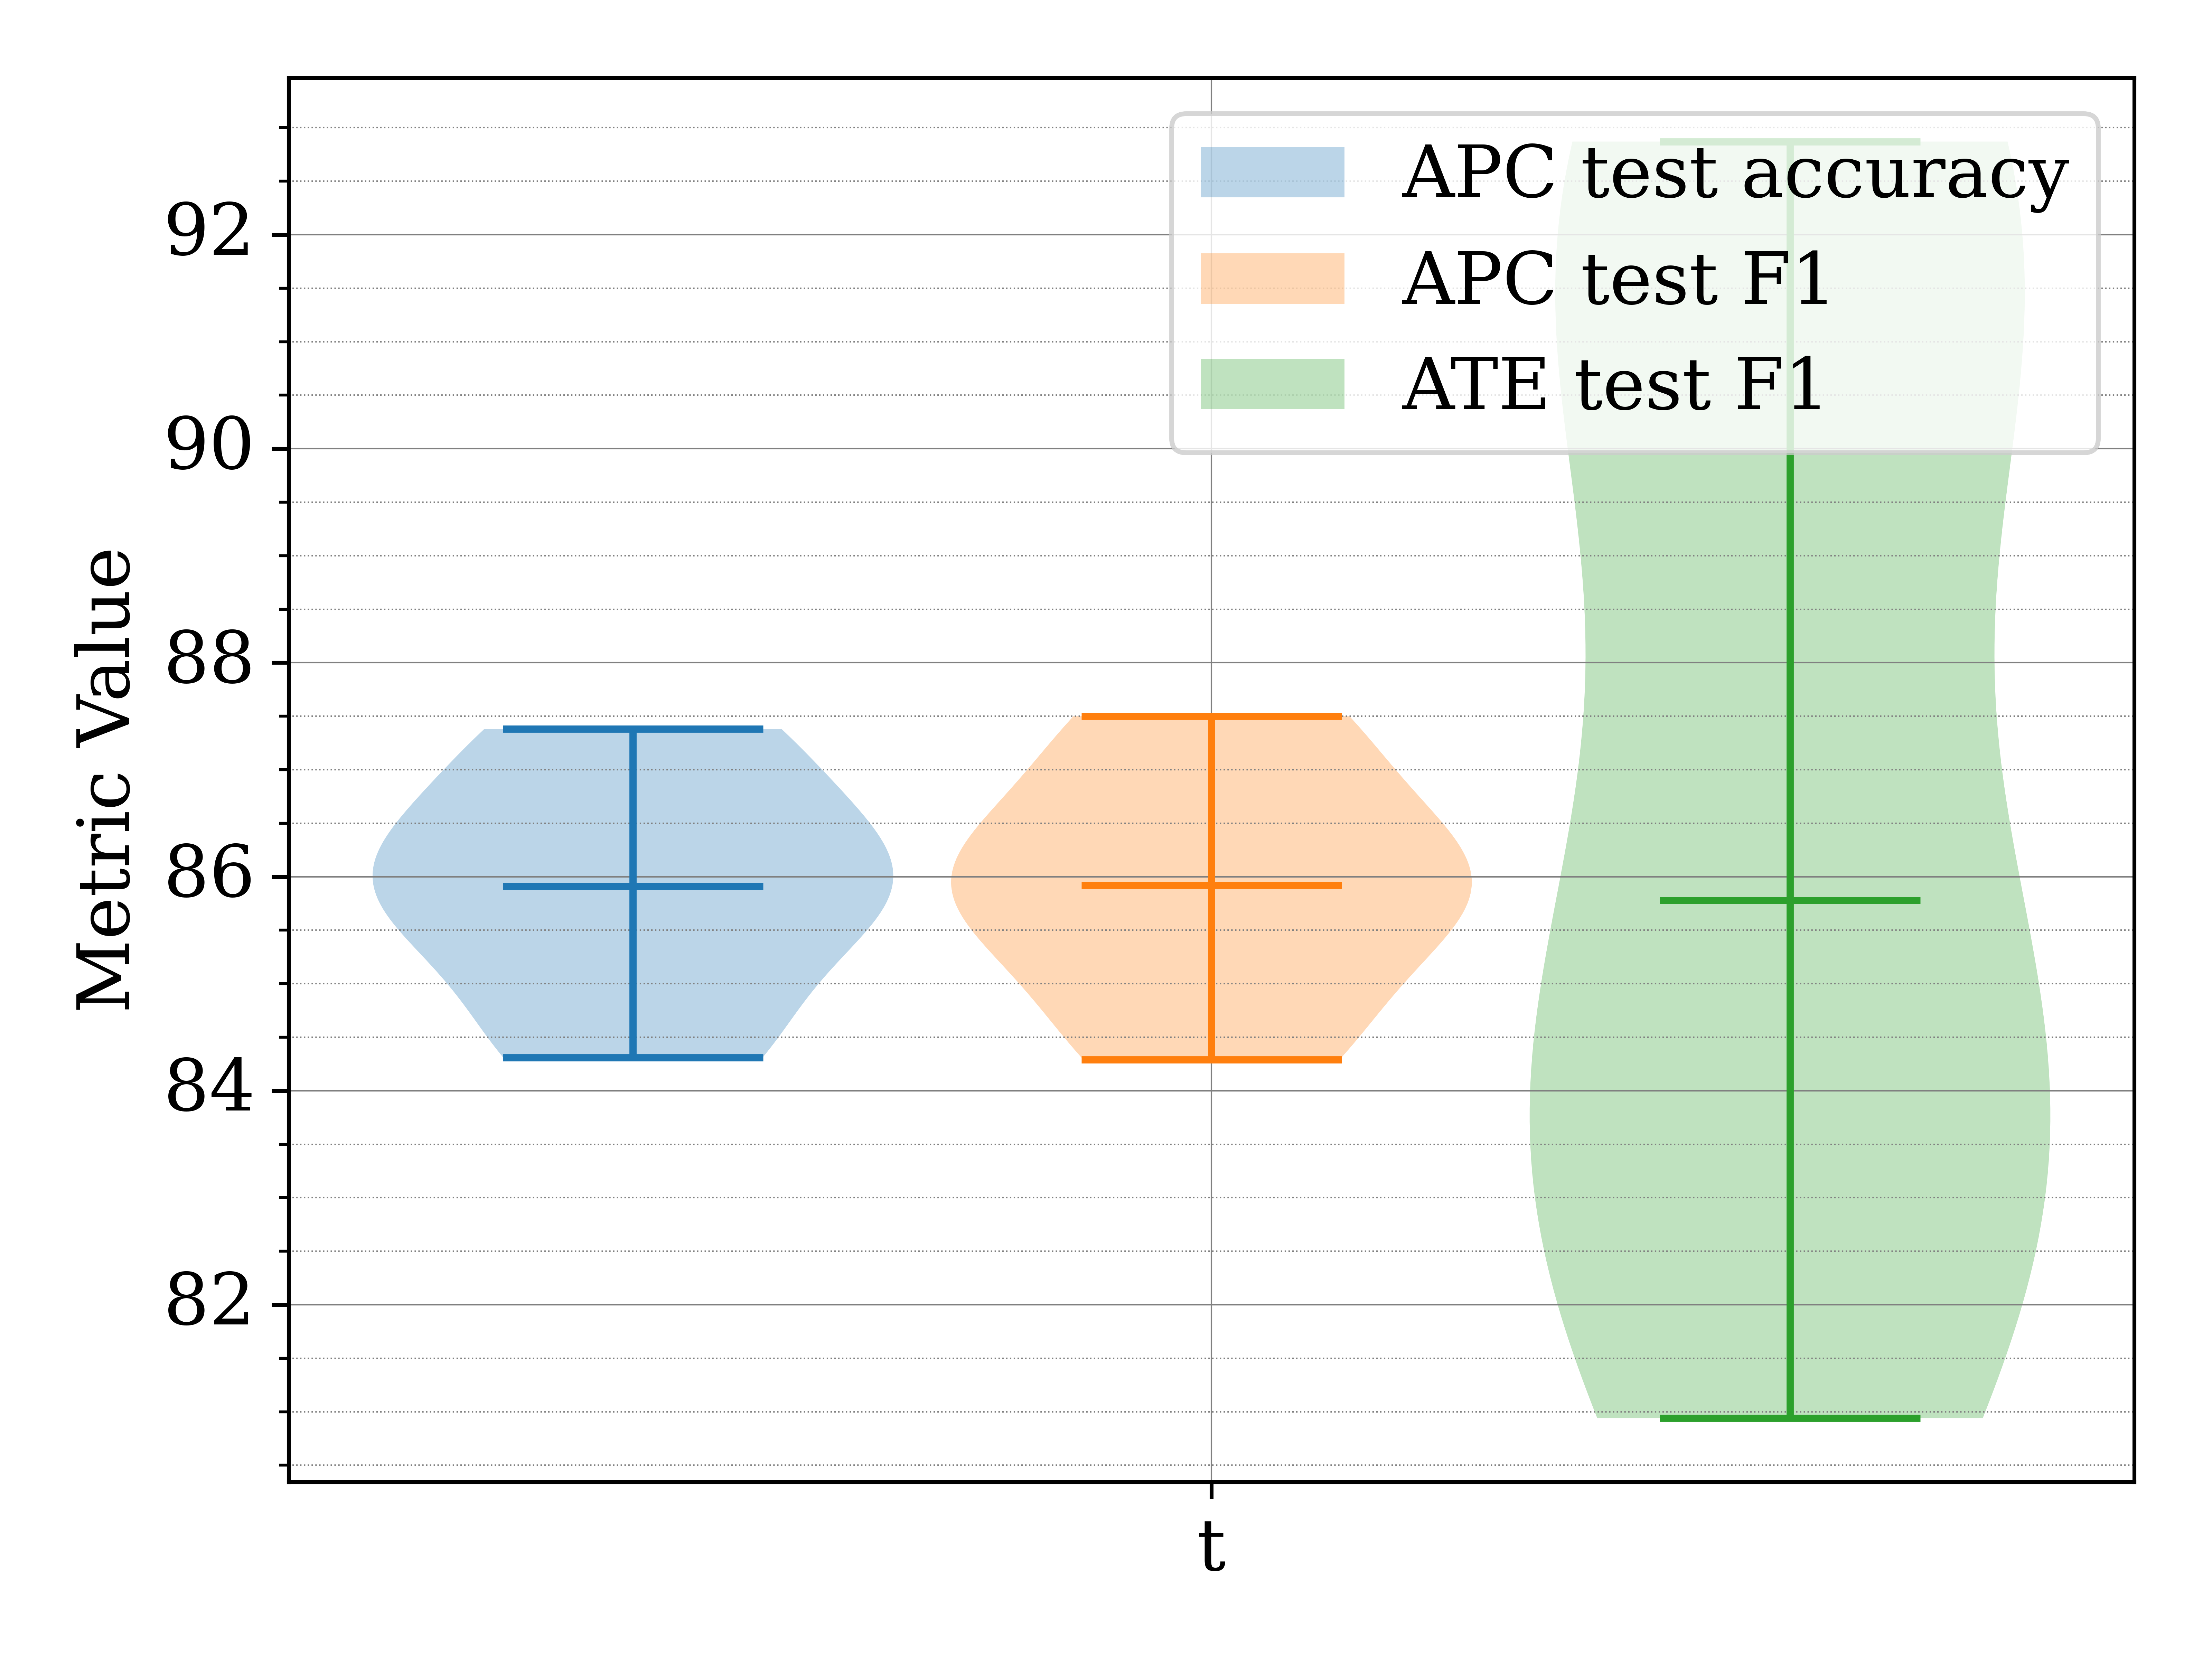
\includegraphics[width=1\linewidth]{images/violin_plot03.png}
    \caption{Скрипичный график всех моделей на одном графике}
    \label{fig:violin-plot}
\end{figure}

На рисунке 4 видно, что распределение точности на тестовой выборке в задаче классификации  эмоциональной окраски текста APC (синий цвет, см. рис. ~\ref{fig:violin-plot}) является относительно компактным с центром значений около 86-87\%. Аналогично, распределение F1-меры по задаче APC является относительно компактным с центром значений около 85-86\%. Оба распределения указывают на стабильную производительность модели для задачи APC, с минимальной изменчивостью, что нельзя сказать о распределении F1 модели для задачи ATE, у которой распределение значительно шире, что свидетельствует о большей изменчивости в производительности. Центр распределения находится около 86\%, но значительный разброс указывает на то, что производительность может значительно варьироваться по сравнению с метриками APC. Если рассматривать только точности трех моделей, получаем следующие значения (~\ref{tabl:5}): 

\begin{center}
\begin{table}[h!]
\centering
\caption{Максимальная точность модели в задаче ATE\textunderscore APC}
\label{tabl:5}
\begin{tabular}{|c|c|}
\hline
~~~~max\textunderscore seq\textunderscore len~~~~&~~~~точность~~~~\\
\hline
60  &	86.40\%\\
\hline
80  &	87.38\%\\
\hline
100  &	87.30\%\\
\hline
\end{tabular}
\end{table}
\end{center}

Фреймворк pyABSA позволяет нам сохранить модель после обучения. При помощи метода predict можно предсказать оценку тональности и объект этой тональности. К примеру, используем следующее предложение \flqq Apple stocks went up by 10 \% on Monday, according to TASS\frqq. Это предложение сложное по структуре, так как в нем два объекта тональности Apple и TASS. Модель выводит следующую информацию:

\begin{lstlisting}[label=listing8, caption=Predication, language = Python]
[{"sentence": "Apple stocks went up by 10 % on Monday , according to TASS .", 
"IOB": ["B-ASP", "O", "O", "O", "O", "O", "O", "O", "O", "O", "O", "O", "O", "O"], 
"tokens": ["Apple", "stocks", "went", "up", "by", "10", "%", "on", "Monday", ",", "according", "to", "TASS", "."], 
"aspect": ["Apple"], 
"position": [[0]], 
"sentiment": ["Positive"], 
"probs": [[0.008858616463840008, 0.16175325214862823, 0.8293880820274353]], 
"confidence": [0.8294]}]
\end{lstlisting}

Модель смогла только правильно определить первую сущность Apple  и правильнную тональность относительно Apple, но не смогла определить вторую сущность TASS. Это один из недостатков модели, она плохо распознает и извлекает сущности в тексте, если их больше одной. Иногда не распознает даже ни одну из сущностей. Например, в  \flqq Saudi’s Biggest Listing of the Year Fakeeh Rises in Riyadh Debut\frqq \vspace{1pt} Saudi, Fakeeh Rises и Riyadh Debut - это сущности в тексте модель не смогла извлечь даже одну из них.
\begin{lstlisting}[label=listing8, caption=No Predication, language = Python]
[{"sentence": "Saudi ’ s Biggest Listing of the Year Fakeeh Rises in Riyadh Debut", 
"IOB": ["O", "O", "O", "O", "O", "O", "O", "O", "O", "O", "O", "O", "O"], 
"tokens": ["Saudi", "’", "s", "Biggest", "Listing", "of", "the", "Year", "Fakeeh", "Rises", "in", "Riyadh", "Debut"], 
"aspect": [], 
"position": [], 
"sentiment": [], 
"probs": [], 
"confidence": 
[]}]
\end{lstlisting}

\begin{lstlisting}[label=listing8, caption=No Predication, language = Python]
[{"sentence": "Treasury rubbishes Rishi Sunak ’ s £ 2 , 000 tax hike election TV debate claim", "IOB": ["O", "O", "O", "O", "O", "O", "O", "O", "O", "O", "O", "O", "O", "O", "O", "O"], "tokens": ["Treasury", "rubbishes", "Rishi", "Sunak", "’", "s", "£", "2", ",", "000", "tax", "hike", "election", "TV", "debate", "claim"], 
"aspect": [], 
"position": [], 
"sentiment": [], 
"probs": [], 
"confidence": []}]
\end{lstlisting}
\begin{lstlisting}{lstlisting}[label=listing9, caption=No Predication, language = Python]
[{"sentence": "Russia Oil Revenue Rose 50 % in May as Nation Adapts to Sanctions", 
"IOB": ["O", "O", "O", "O", "O", "O", "O", "O", "O", "O", "O", "O", "O"], 
"tokens": ["Russia", "Oil", "Revenue", "Rose", "50", "%", "in", "May", "as", "Nation", "Adapts", "to", "Sanctions"], 
"aspect": [], 
"position": [], 
"sentiment": [], 
"probs": [], 
"confidence": []}]
\end{lstlisting}

Модель также не может распознать сарказм и шутки потому, что в финансовых новостях шутки как правило не используются, а, соответственно, она не склонна их извлекать в принципе.
\vfill
\begin{lstlisting}{lstlisting}[label=listing10, caption=Sarcasm, language = Python]
[{"sentence": "Market Rejoices as Investors Discover New Trend : Losing Money Faster Than Ever Before !", 
"IOB": ["O", "O", "O", "O", "O", "O", "O", "O", "O", "O", "O", "O", "O", "O", "O"], 
"tokens": ["Market", "Rejoices", "as", "Investors", "Discover", "New", "Trend", ":", "Losing", "Money", "Faster", "Than", "Ever", "Before", "!"], 
"aspect": [],
"position": [],
"sentiment": [], 
"probs": [], 
"confidence": []}]
\end{lstlisting}

Помимо вышесказанного, особенность fine\textunderscore tuned модели BERT - плохая работоспособность на данных, на которых модель не была дополнительно обучена. Этот феномен называется Model Sensitivity в сфере NLP и трансформеров. 

\section{Выводы}

За период практики, которую я проходил на кафедре математического моделирования и искусственного интеллекта факультета физико-математических и естественных наук РУДН, были достигнуты все цели и решены все поставленные задачи, определенные в программе преддипломной практики направления подготовки 02.03.01 «Математика и компьютерные науки» (см. введение отчета по практике).
При прохождении практики я разобрался с научной терминологией области исследований; научился осуществлять сбор, анализ и обработку данных, необходимых для решения профессиональных задач; собирать, обрабатывать и интерпретировать данные современных научных исследований, необходимые для формирования выводов по соответствующим научным исследованиям; осуществлять целенаправленный поиск информации о новейших научных и технологических достижениях в сети Интернет и из других источников; строить и анализировать математические модели объекта исследований; разрабатывать и отлаживать вспомогательные программные комплексы; проводить численный эксперимент; оформлять результаты своих исследований. Также я овладел необходимым математическим и программным аппаратом исследований; навыками математического моделирования, применения численных методов для выполнения необходимых расчетов и получения численных оценок по теме исследований.
В результате прохождения данной практики я приобрел следующие практические навыки, умения, универсальные и профессиональные компетенции:
\begin{itemize}
\item способностью к самоорганизации и к самообразованию;
\item способностью решать стандартные задачи профессиональной деятельности на основе информационной и библиографической культуры с применением информационно-коммуникационных технологий и с учетом основных требований информационной безопасности;
\item способностью к самостоятельной научно-исследовательской работе;
\item способностью находить, анализировать, реализовывать программно и использовать на практике математические алгоритмы, в том числе с применением современных вычислительных систем;
\item способностью к определению общих форм и закономерностей отдельной предметной области;
\item способностью математически корректно ставить естественнонаучные задачи, знание постановок классических задач математики;
\item способностью строго доказать утверждение, сформулировать результат, увидеть следствия полученного результата;
\item способностью публично представлять собственные и известные научные результаты;
\item способностью использовать методы математического и алгоритмического моделирования при решении теоретических и прикладных задач; 
\item способностью передавать результат проведенных физико-математических и прикладных исследований в виде конкретных рекомендаций, выраженной в терминах предметной области изучавшегося явления;
\item способностью представлять и адаптировать знания с учетом уровня аудитории;
\item способностью к проведению методических и экспертных работ в области математики.
\end{itemize}

Выполненный во время проведения преддипломной практики обзор публикаций научных изданий как по теме Обработка естественного языка NLP, так и по теме анализа тональности текста и по теме технологии трасормеров таких как BERT от Google и GPT от Open AI, позволит мне обосновать актуальность выбранной темы, а также более полно раскрыть постановку задачи и методы исследования при написании выпускной квалификационной работы бакалавра.


%\input{lab2} Отчёт к каждой работе оформляется в отдельном файле
\addcontentsline{toc}{section}{Список литературы} % Add bibliography to table of contents
\printbibliography % Command to print the bibliography

\end{document}
